%\documentclass[11pt, letterpaper, twoside, openright]{book}
\documentclass[11pt]{article}
\usepackage[margin=1in]{geometry}
\usepackage{tikz}

\usepackage{array} % center alignment within columns
\usepackage{multirow} % to merge rows in column

\usepackage{enumerate} % lists (a), (b), (c), ...

\usepackage{framed}
\usepackage[framemethod=TikZ]{mdframed}

\usepackage{amsmath} % for align environment
\usepackage{mathtools}% Loads amsmath \\ % for \underbrace \overbrace
\usepackage{amsthm} % for proofs
\usepackage{amssymb} % Symbols - black square
\renewcommand\qedsymbol{$\blacksquare$}

% \renewcommand{\vec}[1]{\mathbf{#1}} %This command will make \vec typeset LaTeX vectors using bold instead of an arrow:
\renewcommand{\vec}[1]{\underline{#1}} % This command will make \vec typeset LaTeX vectors using an underline (vandy style)


\usepackage[super]{nth} % 1st, 2nd, 3rd = \nth{1}, \nth{2}, \nth{3}

\usepackage{multicol} % For columns in text

\usepackage{graphicx}
\usepackage{float} % Here dammit! \begin{figure}[H]
\usepackage{caption} % \cation*{Name} for figure removes numbering

\begin{document}

\begin{center}
	\def \firstcircle{(0,0) circle (1)}
	\def \secondcircle{(1,0) circle (1)}
\begin{tabular}{ >{\centering\arraybackslash}m{1in} 
			>{\centering\arraybackslash}m{1.5in} 
			>{\centering\arraybackslash}m{2in} } 
\textbf{Subset} \hspace{3in} $A \in B$
&
if $x\in A$ then $x \in B$
&
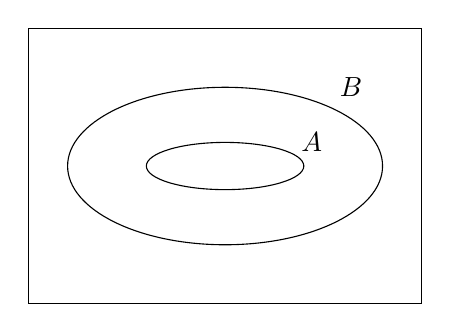
\begin{tikzpicture}
	\draw (0,0) ellipse (2 and 1) (1.6, 1) node {$B$};
	\draw (0,0) circle (1 and 0.3) (1.1, 0.3) node {$A$};
	\draw (-2.5, -1.75) rectangle (2.5,1.75);
\end{tikzpicture}
\\
\textbf{Union} \hspace{3in} $A \cup B$ 
& $\left\{ x: x\in A \textrm{ or } x \in B\right\}$
& 
\begin{tikzpicture}
	\draw \firstcircle (0,1) node[text=black,above]  {$A$}; 
	\draw \secondcircle (1, 1) node[above] {$B$};
	\begin{scope}[fill opacity = 0.5]
		\fill[gray] \firstcircle \secondcircle;
	\end{scope}
	\draw (-1.5,-1.5) rectangle (2.5, 1.75);
\end{tikzpicture}
\\
\textbf{Intersection} \hspace{3in} $A \cap B$
&  $\left\{ x: x\in A \textrm{ and } x \in B\right\}$
&
\begin{tikzpicture}
	\draw \firstcircle (0,1) node[text=black,above]  {$A$}; 
	\draw \secondcircle (1, 1) node[above] {$B$};
	\begin{scope}[fill opacity = 0.5]
		\clip \firstcircle;  
		\fill[gray] \secondcircle;
	\end{scope}
	\draw (-1.5,-1.5) rectangle (2.5, 1.75);
\end{tikzpicture}
\\
\textbf{Complment} \hspace{3in} $A^{C}$
&  $\left\{ x: x\notin A\right\}$
&
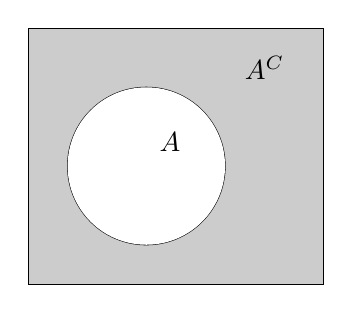
\begin{tikzpicture}
	\filldraw[fill=gray, fill opacity = 0.4] 
		(-1.5,-1.5) rectangle (2.25, 1.75);
	\draw (0,0) circle (1);
	\begin{scope}[white]
		\clip (-1.5,-1.5) rectangle (2.25, 1.75);
		\fill (0,0) circle (1);
	\end{scope}
	% \draw (-1.5,-1.5) rectangle (2.5, 1.75);
	\draw (1.5, 1.25) node {$A^{C}$}
		  (0.3, 0.3) node {$A$};
\end{tikzpicture}
\\
%\textbf{Disjoint} \hspace{3in} $A \cap B = \emptyset$
% &  \textbf{Pairwise Disjoint} $A_{i} \cap A_{j} = \emptyset$ \hspace{3in} for all $i \neq j$
& 
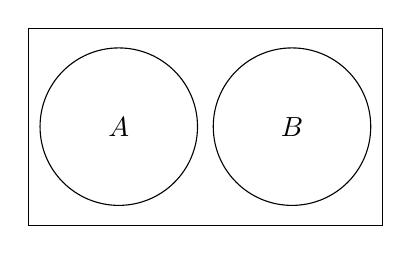
\begin{tikzpicture}
	\draw (-1.1,0) circle (1) node {$A$}
		(1.1,0) circle (1) node {$B$};
	\draw (-2.25,-1.25) rectangle (2.25, 1.25);
\end{tikzpicture}
\\
%\textbf{Pairwise Disjoint}
%&  $A_{i} \cap A_{j} = \emptyset$ \hspace{3in} for all $i \neq j$
%& 
%\begin{tikzpicture}
%	\draw (-1.1,-0.5) circle (0.75) node {$A$}
%		 (0, 0.8) circle (0.75) node {$B$}
%		 (1.1, -0.5) circle (0.75) node {$C$};
%	\draw (-2.25,-1.5) rectangle (2.25, 1.75);
%\end{tikzpicture}
\textbf{Partition}
& If $A_{1}, A_{2}, \dots$ are pairwise disjoint and $\cup_{i=1}^{\infty} A_{i} = S$, then the collection $A_{1}, A_{2}, \dots$ forms a partition of S.
&
\begin{tikzpicture}
	\draw (-2.25, -1.5) rectangle (2.25, 1.5);
	\draw (-0.75, -1.5) -- (-0.75, 1.5)
		  (0.75, -1.5) -- (0.75, 1.5);
	\draw (-1, 1) node {$A$}
		  (0.5, 1) node {$B$}
		  (2, 1) node {$C$}
		  (2.5, 1.5) node {$S$};
\end{tikzpicture}
\end{tabular}
\end{center}

\newpage
\noindent\textbf{Theorems}
\begin{enumerate}[(a)]
\item $P(B \cap A^C) = P(B) - P(A \cap B)$
\begin{multicols}{2}
\begin{proof}
	\begin{align*}
	B &= (B \cap A^C) \cup (B \cap A) \\
	P(B) &= P(B \cap A^C) \cup P(B \cap A) \\
	\Rightarrow P(B \cap A^C) &= P(B) - P(B \cap A)
	\end{align*}
\end{proof}
\columnbreak % omit and columns balance automatically
\begin{center}
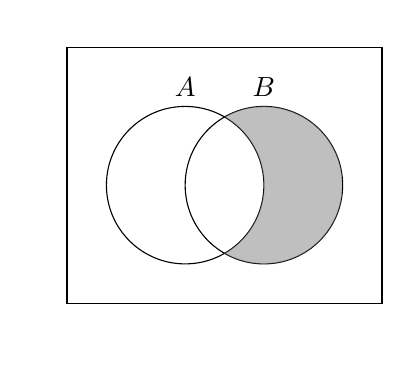
\begin{tikzpicture}
	\draw (0,0) circle (1) (0,1) node[text=black,above]  {$A$}; 
	\draw (1,0) circle (1) (1, 1) node[above] {$B$};
	\begin{scope}[fill opacity = 0.5]
		\clip (0,0) circle (1) (-2, -2) rectangle (2, 2);
		\fill[gray] (1,0) circle (1);
		% \clip (0,0) circle (1) (0,1); 
		%\fill[gray] (1,0) circle (1) (1, 1);
		%\clip (0,0) circle (1) (0,1);
	\end{scope}
	\draw (-1.5,-1.5) rectangle (2.5, 1.75);
\end{tikzpicture}
\end{center}
\end{multicols}
\item $P(A \cup B) = P(A) + P(B) - P(A \cap B)$
\begin{multicols}{2}
\begin{proof}
	\begin{align*}
	A \cup B &= A \cup (B \cap A^C) \\
	P(A \cup B) &= P(A) + P(B \cap A^C) \\
	&= P(A) + P(B) - P(B \cap A)
	\end{align*}
\end{proof}
\columnbreak % omit and columns balance automatically
\vspace*{20pt}
%\vspace*{\textheight}
\end{multicols}
\item $A \in B \Rightarrow P(A) \leq P(B)$
\begin{multicols}{2}
\begin{proof}
	\begin{align*}
	A &= A \cap B \\
	P(A) &= P(A \cap B) \\
	P(B) &= P(B \cap A^C) + P(B \cap A) \\
	&= P(B \cap A^C) + P(A) \\
	P(B) \geq P(A)
	\end{align*}
\end{proof}
\columnbreak % omit and columns balance automatically
\begin{center}
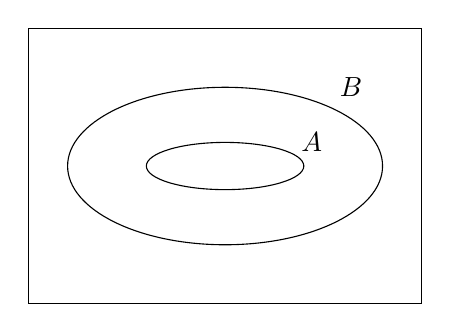
\begin{tikzpicture}
	\draw (0,0) ellipse (2 and 1) (1.6, 1) node {$B$};
	\draw (0,0) circle (1 and 0.3) (1.1, 0.3) node {$A$};
	\draw (-2.5, -1.75) rectangle (2.5,1.75);
\end{tikzpicture}
\end{center}
\end{multicols}
\end{enumerate}


\end{document}